\subsection{Nebulas Virtual Machine (NVM)}
\label{sec:nvm}

We will introduce LLVM \cite{llvm} as the main component of NVM and
LLVM bytecode as the NVM bytecode. The NVM bytecode is dynamically
compiled and optimized through LLVM JIT and is executed in the NVM sandbox environment. With this architecture design, the performance and security of the core code and the smart contract of Nebulas can be continuously improved with the introduction of LLVM.

LLVM is a collection of highly modularized compiler toolchains and
technologies, which was used as a code compilation framework in Google, Apple
and many other companies. LLVM provides neutral intermediate representations
(LLVM IR) and the corresponding compilation infrastructure, and offers a brand
new set of compilation strategies regard to these infrastructure, including
optimization of LLVM IR, code generation from the LLVM IR to the LLVM bytecode
and direct execution of the LLVM bytecode in different hardware platforms via
the LLVM JIT, shown in \reffig{fig:llvm}. \\

\begin{figure}[h]
\centering
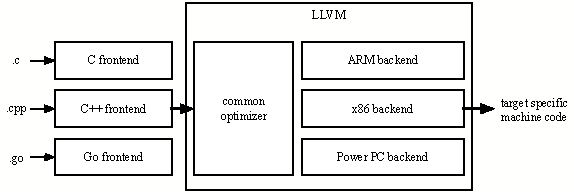
\includegraphics[width=10cm]{./figs/llvm}
\caption{LLVM}
\label{fig:llvm}
\end{figure}

We construct the NVM based on LLVM, shown in \reffig{fig:nvm}. First
of all, we provide the underlying API libraries for blockchains. After that, we
construct compiler frontend for different languages, such as Solidity,
JavaScript, C/C ++, Go, etc. Then, we use the toolchain provided by LLVM to
generate the LLVM bytecode. Finally, the LLVM bytecode is executed in a safe
sandbox environment provided by NVM through JIT engine of LLVM.

\begin{figure}[h]
\centering
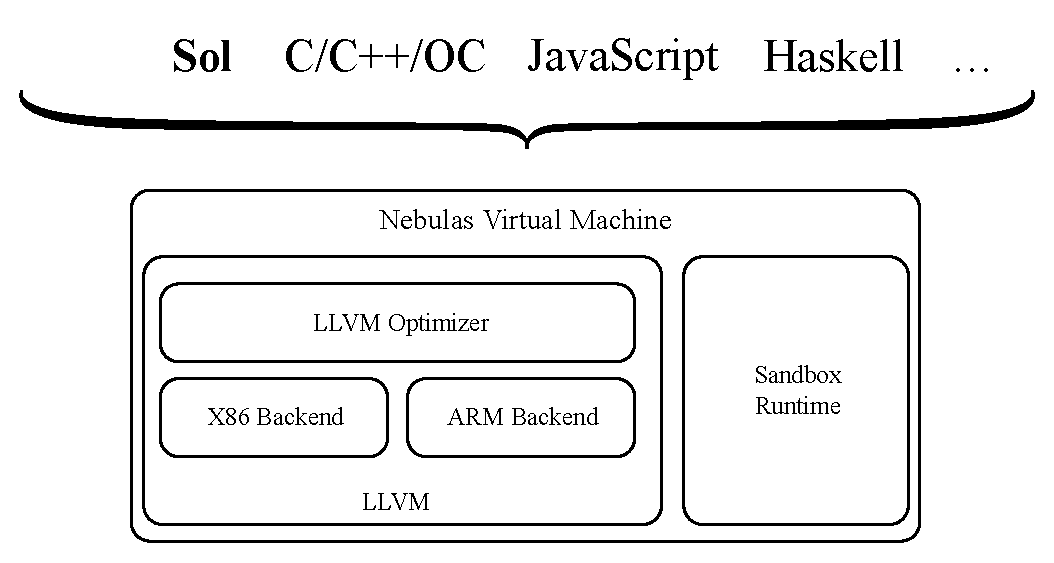
\includegraphics[width=10cm]{./figs/nvm}
\caption{Nebulas Virtual Machine}
\label{fig:nvm}
\end{figure}

NVM is an important cornerstone of the Nebulas Force. When any new protocol
code or smart contract is released, the LLVM bytecode is generated after the
new code is complied by the LLVM compiler module in NVM and is released to the
chain. After confirmed on chain, the new code will be complied and
optimized by LLVM JIT, and then into the sandbox to replace the old code and
be executed, shown in \reffig{fig:nvm-process}.

\begin{figure}[h]
\centering
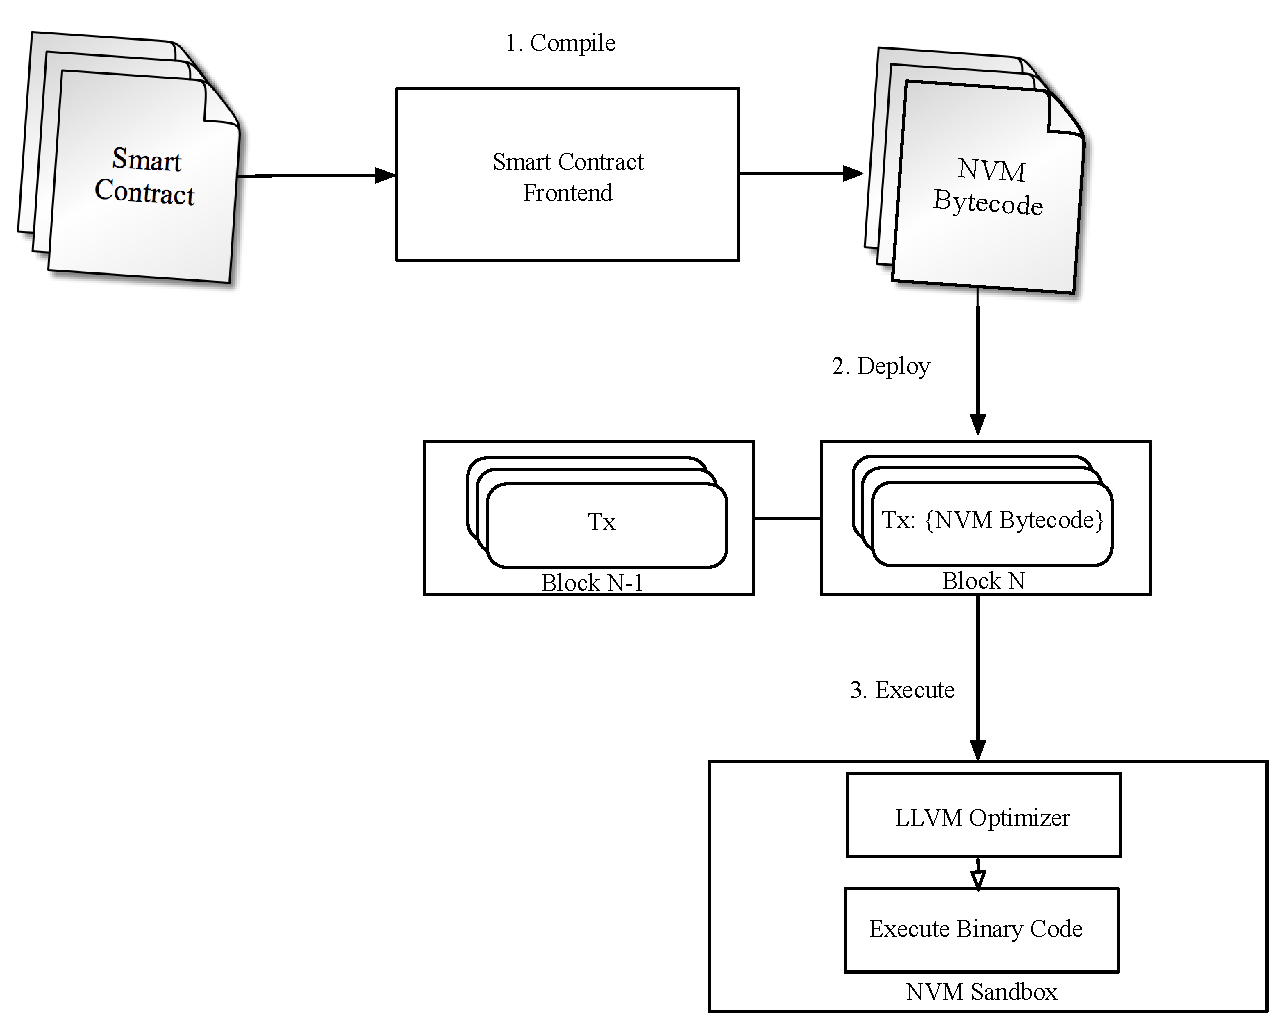
\includegraphics[width=10cm]{./figs/nvm-process}
\caption{The operation mechanism of the Nebulas Virtual Machine}
\label{fig:nvm-process}
\end{figure}

With LLVM (see \reffig{fig:llvm}), NVM also supports developers to develop
smart contracts and applications with their familiar programming languages,
such as Solidity, more flexible JavaScript, and even pure functions type of
language Haskell. In addition to these popular languages, NVM can also provide
customized high-level languages for different areas and scenarios, such as DSL
(domain-specific language) for financial systems. These high-level languages
are easier to be formally verified, further improving code robustness and
security, and more conducive to the developers developing richer Smart contract
and application.